\documentclass[9pt, aspectratio=169]{beamer}

\usetheme{metropolis}
\setbeamertemplate{itemize items}{\faAngleRight}

\metroset{titleformat=smallcaps,block=fill,numbering=counter,progressbar=frametitle,sectionpage=none}
\setbeamersize{text margin left=5mm,text margin right=5mm} 
% \input{embed_video}
\usepackage{fontspec,minted}
\usepackage[scale=1]{ccicons}
\usepackage{metalogo}
\usepackage{xcolor,colortbl}
\usepackage{multicol,multirow,booktabs}
\usepackage{appendixnumberbeamer}
\usepackage{graphicx}
\usepackage{mismath}
\usepackage{bm}
\usepackage{fontawesome5}
\usepackage{csquotes}
\usepackage[backend=biber, natbib, sorting=nyt, doi=true, url=false, url=false, isbn=false, maxbibnames=10]{biblatex}
\addbibresource{../utils/refs.bib}

\usepackage[spanish, es-nodecimaldot]{babel}
\deftranslation[to=spanish]{Definition}{Definición}
\deftranslation[to=spanish]{Theorem}{Teorema}
\deftranslation[to=spanish]{Example}{Ejemplo}

\usepackage{mathtools, mathrsfs}
\usefonttheme{professionalfonts}
\usepackage{textcomp, wasysym}

\setsansfont[BoldFont={Iwona Heavy}, Numbers={Lining, Proportional}]{Iwona Light}
\setmonofont[Scale=MatchLowercase]{Hack Nerd Font Mono}

\setbeamercolor{alerted text}{fg=red,bg=black!2}
\setbeamercolor{progress bar}{fg=red,bg=red!2}
\setbeamertemplate{itemize item}{\faCaretRight}
\setbeamertemplate{itemize subitem}{ \faAngleRight}
\setbeamertemplate{blocks}[shadow=false]
\setbeamercolor{block title}{bg=black!30,fg=red}
\setbeamercolor{block body}{bg=black!20,fg=black}
\setbeamertemplate{theorem begin}
{%
\begin{\inserttheoremblockenv}
{%
\inserttheoremheadfont
%{Teorema:}
\inserttheoremname
\ifx\inserttheoremaddition\@empty\else\ : \inserttheoremaddition\fi%
\inserttheorempunctuation
}%
}
\setbeamertemplate{theorem end}{\end{\inserttheoremblockenv}}
\makeatother


 
\usepackage{gensymb,amssymb}
\usepackage{siunitx}
\DeclareSIUnit{\nada}{\relax}
\usepackage{upquote}
\usepackage{cancel}
\usepackage{algpseudocode}
\algrenewcommand\algorithmicrequire{\textbf{Requiere}}
\algrenewcommand\algorithmicensure{\textbf{Devuelve}}
\setbeamertemplate{blocks}[shadow=false]

\newcommand{\cx}{\column{0.5\textwidth}}
\newcommand{\cw}[1]{\column{#1\textwidth}}

\author{Manuel Carlevaro}
\date{{\tiny Departamento de Ingeniería Mecánica \\
             Grupo de Materiales Granulares - UTN FRLP \\
             manuel.carlevaro@gmail.com }}
\institute{
  \vspace{6em}
  \centering
  {\tiny
  Cálculo Avanzado \enspace • \enspace 2025 \\
    \faLinux \- $\cdot$ \- \fontspec{TeX Gyre Pagella}\XeLaTeX \- $\cdot$ \- \ccbysa }
}

%% Operadores
\DeclareMathOperator{\sen}{sen}
\DeclareMathOperator{\senc}{senc}
\DeclareMathOperator{\sign}{sign}
\DeclareMathOperator{\Tr}{Tr}
\DeclareMathOperator{\rg}{rg}
\DeclareMathOperator{\cond}{cond}
\newcommand{\T}[1]{\underline{\bm{#1}}}
\newcommand{\uvec}[1]{\hat{\bm{#1}}}

\usepackage{hyperref}
\hypersetup{
    colorlinks,
    citecolor=blue,
    filecolor=black,
    linkcolor=blue,
    urlcolor=blue
}
\urlstyle{same}

%% Códigos
\usepackage{minted}
\newminted[cpp]{cpp}{linenos,fontsize=\footnotesize,frame=lines,numbersep=4pt}
\newmintedfile[cppcode]{cpp}{linenos,fontsize=\footnotesize,frame=lines,numbersep=4pt}
\newcommand{\mic}[1]{\mintinline{C++}{#1}}

\newminted[py]{python}{linenos,fontsize=\footnotesize,frame=lines,numbersep=4pt}
\newminted[pyc]{pycon}{linenos,fontsize=\footnotesize,frame=lines,numbersep=4pt} % Consola de Python
\newminted[ipy3]{ipython3}{linenos,fontsize=\footnotesize,frame=lines,numbersep=4pt} % Consola de iPython3
\newmintedfile[pycode]{python}{linenos,fontsize=\footnotesize,frame=lines,numbersep=4pt}

\newmintedfile[makef]{basemake}{linenos,fontsize=\footnotesize,frame=lines,numbersep=4pt}
\definecolor{bg}{RGB}{22,43,58}
\newminted[shell]{console}{linenos=false,fontsize=\footnotesize,breaklines=true, frame=single} % Linea de comandos
\renewcommand\listingscaption{Código}

\makeatletter
\AtBeginEnvironment{minted}{\dontdofcolorbox}
\def\dontdofcolorbox{\renewcommand\fcolorbox[4][]{##4}}
\makeatother

% uso:
% Ejemplo de uso explícito:
% \begin{py}
% >>> list("abcd")
% ['a', 'b', 'c', 'd']
% \end{py}
% 
% Ahora ejemplo de código en file:
% \pycode{Chapters/intro/code/hola.py}
% 
% También se puede poner un sector del file:
% \pycode[firstline=6, lastline=7]{Chapters/intro/code/hola.py}
% 
% También se puede poner código \textit{inline}: \mip{print('¡Hola mundo!')} y en una sola línea:
% \slp|if __name__ == '__main__')|
% 
% Por último, se puede poner el código en un entorno \textit{float}, esto es, como las tablas y las figuras, con un caption y un label para luego hacer referencias, como por ejemplo al Código \ref{code:hola}.


\usepackage{tikz}
\usetikzlibrary{shapes,shadows,arrows,positioning,matrix,chains,backgrounds,fit}

\tikzset{
    %Define standard arrow tip
    >=stealth',
    %Define style for boxes
    obj/.style={
           rectangle,
           rounded corners,
           draw, very thick,
           text width=10em, fill=green!20,
           minimum height=2em,
           text centered, drop shadow},
    proc/.style={
	    rectangle, rounded corners,
	    draw,fill=red!50,very thick,
	    text width=8em,minimum height=2em,
	    text centered, drop shadow},
    % Define arrow style
    pil/.style={
           ->,
           thick,
           shorten <=2pt,
           shorten >=2pt,}
}

\setbeamertemplate{bibliography item}{%
  \ifboolexpr{ test {\ifentrytype{book}} or test {\ifentrytype{mvbook}}
    or test {\ifentrytype{collection}} or test {\ifentrytype{mvcollection}}
    or test {\ifentrytype{reference}} or test {\ifentrytype{mvreference}} }
    {\setbeamertemplate{bibliography item}{\faBook}}
    {\ifentrytype{online}
            {\setbeamertemplate{bibliography item}{\faGlobe}}
   {\setbeamertemplate{bibliography item}{\faFileText}}}%
  \usebeamertemplate{bibliography item}}

\defbibenvironment{bibliography}
  {\list{}
     {\settowidth{\labelwidth}{\usebeamertemplate{bibliography item}}%
      \setlength{\leftmargin}{\labelwidth}%
      \setlength{\labelsep}{\biblabelsep}%
      \addtolength{\leftmargin}{\labelsep}%
      \setlength{\itemsep}{\bibitemsep}%
      \setlength{\parsep}{\bibparsep}}}
  {\endlist}
  {\item}
\newcommand{\bcite}[1]{\citeauthor{#1}, \citetitle{#1} (\citeyear{#1})}

\usepackage{animate}
\addbibresource{../utils/refs.bib}
\input{embed_video}

\title{Ecuaciones diferenciales parciales de segundo orden}
\subtitle{}

%%%%
% Bibliografía
% Nakamura
% Kreyszig Chap 21
% Epperson Chap. 9
%%%%

\begin{document}
\maketitle

\begin{frame}
    \textbf{Ecuación diferencial parcial (EDP) lineal de segundo orden:}
    \[ A \frac{\partial^2 \phi}{\partial x^2} + B \frac{\partial^2 \phi}{\partial x \partial y} + C \frac{\partial^2 \phi}{\partial y^2} + D \frac{\partial \phi}{\partial x} + E \frac{\partial \phi}{\partial y} + F \phi = S \]
donde $A, B, C, D, E, F$ y $S$ son funciones de $x$ y $y$ en $D \in \R^2$.
\vspace{2em}
\pause

\begin{columns}[t]
\cx
\textbf{Tipos:}
\begin{itemize}
\item \alert<2> {Parabólica: $B^2 - 4 A C = 0$}
\item \alert<3> {Elíptica: $B^2 - 4 A C < 0$}
\item \alert<4> {Hiperbólica: $B^2 - 4 A C > 0$}
\end{itemize}
para todo $(x, y) \in D$.

\cx
\textbf{Casos:}
\only<2> {
    \begin{itemize}
        \item Conducción de calor en sólidos, flujo de fluidos
        \item Ejemplos:
            \begin{itemize}
                \item Conducción de calor:
                    \[ \rho c \frac{\partial T}{\partial t} = k \frac{\partial^2 T(x, t)}{\partial x^2} + Q(x) \]
                \item Transporte convectivo:
                    \[ \frac{\partial \phi}{\partial t} = -\frac{\partial}{\partial x} u(x) \phi + D \frac{\partial^2 \phi}{\partial x^2} \]
            \end{itemize}
    \end{itemize}
}
\only<3> {
    \begin{itemize}
        \item Problemas estacionarios de 2 y 3 dimensiones
        \item Conducción de calor en sólidos, vibración de membranas
        \item Ejemplos:
            \begin{itemize}
                \item Ecuación de Poisson:
                    \[ -\nabla^2 \phi(x, y) = S(x, y) \]
                \item Ecuación de Laplace:
                    \[ -\nabla^2 \phi(x, y) = 0 \]
            \end{itemize}
    \end{itemize}
}
\only<4> {
    \begin{itemize}
        \item Problemas oscilatorios, propagación de ondas, fluidos
        \item Ejemplos:
        \begin{itemize}
            \item Ecuación de onda:
                \[ \frac{\partial^2 u(x, y, z, t)}{\partial t^2} = c^2 \nabla^2 u(x, y, z, t) \]
            \item Navier-Stokes (incompresible):
                \[ \frac{\partial \bm{u}}{\partial t} + (\bm{u} \cdot \nabla) \bm{u} - \nu \nabla^2 \bm{u} = -\nabla \left( \frac{p}{p_0} \right) + \bm{g} \] 
        \end{itemize}
    \end{itemize}
}
\end{columns}
\end{frame}

\begin{frame}
\textbf{Ecuación de Poisson (elíptica):}
\[ \nabla^2 u(x, y) = \frac{\partial^2 u}{\partial x^2}(x, y) + \frac{\partial^2 u}{\partial y^2}(x, y) = f(x, y) \]
en $R = \{(x, y) | a < x < b, c < y < d \}$, con $u(x, y) = g(x, y)$ para $(x, y) \in S$, siendo $S$ la frontera de $R$.
\begin{columns}
\cx
\begin{center}
    \includegraphics[scale=0.8]{figs/malla-01.pdf}
\end{center}
\cx
\textbf{Malla:}
\begin{itemize}
    \item División $[a, b]$ y $[c, d]$ en $n$ y $m$ partes iguales
    \item $h = (b - a) / n$, $k = (d - c) / m$
    \item $x_i = a + i h, \; i = 0, 1, \ldots, n$
    \item $y_j = c + j k, \; j = 0, 1, \ldots, m$
\end{itemize}

\textbf{Aproximación en diferencias finitas (serie de Taylor):}
\[ \frac{\partial^2 u}{\partial x^2} = \frac{u(x_{i+1}, y_j) - 2 u(x_i, y_j) + u(x_{i-1},y_j)}{h^2} + \bigO(h^2) \]
\[ \frac{\partial^2 u}{\partial y^2} = \frac{u(x_i, y_{j+1}) - 2 u(x_i, y_j) + u(x_i,y_{j-1})}{k^2} + \bigO(k^2) \]
\end{columns}
\end{frame}

\begin{frame}
    Con $u(x_i, y_j) \mapsto u_{i,j}$:
    \[ \frac{u_{i+1, j} - 2 u_{i,j} + u_{i-1, j}}{h^2} + \frac{u_{i, j+1} - 2 u_{i,j} + u_{i, j-1}}{k^2} = f_{i, j} + \frac{h^2}{12} \frac{\partial^4 u}{\partial x^4}(\xi_i, y_j) + \frac{k^2}{12} \frac{\partial^4 u}{\partial y^4}(x_i, \eta_j) \]
    para $i = 1, 2, \ldots, n-1$, $j = 1, 2, \ldots, m-1$ y condiciones de contorno:
\begin{align*}
    u_{0, j} &= g_{0, j} \txt{y} u_{n, j} = g_{n, j}, \quad j = 0, 1, \ldots m; \\
    u_{i, 0} &= g_{i, 0} \txt{y} u_{i, m} = g_{i, m}, \quad i = 0, 1, \ldots n
\end{align*}
Resulta:
\[ 2 \left[ \pow{\frac{h}{k}}{2} + 1 \right]  u_{i,j} - (u_{i+1, j} + u_{i-1,j}) - \pow{\frac{h}{k}}{2} (u_{i, j+1} + u_{i, j-1}) = -h^2 f_{i,j}, \; i \in [1, n-1], \; j \in [1, m-1] \]
\begin{columns}
\cx
    \begin{center}
        \includegraphics[scale=0.53]{figs/malla-02.pdf}
    \end{center}
\cx
\vspace{1em} \pause

\textbf{Ejemplo:} Determinar la distribución estacionaria de temperaturas en una placa de $0.5 \times 0.5$ m usando $n = m = 4$. Dos bordes adyacentes se mantienen a $0$ \textcelsius{} y la temperatura se incrementa linealmente en los otros bordes hasta llegar a $100$ \textcelsius{} en la esquina de unión.
\end{columns}
\end{frame}

\begin{frame}
\begin{columns}
\cx
\begin{center}
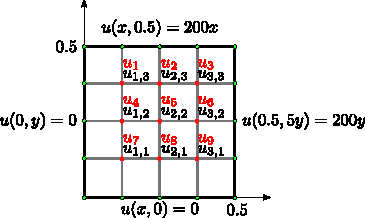
\includegraphics[scale=1.1]{figs/malla-03.pdf}
\end{center}

$u_{i,j} \mapsto u_l,\; l = i + (m - 1 -j) (n - 1) $
\begin{align*}
    u_{1,1} &= u_7,\; u_{2,1} = u_8,\; u_{3,1} = u_{9} \\
    u_{1,2} &= u_4,\; u_{2,2} = u_5,\; u_{3,2} = u_{6} \\
    u_{1,3} &= u_1,\; u_{2,3} = u_2,\; u_{3,3} = u_{2} \\
\end{align*}
\cx
\[ \frac{\partial^2 u}{\partial x^2}(x, y) + \frac{\partial^2 u}{\partial y^2}(x, y) = 0; \;(x, y) \in [0, 0.5]^2 \]
\[ h = k = 1/8 \] \pause
Ecuaciones:
\[ 4 u_{i,j} - u_{i+1, j} - u_{i-1,j} -u_{i,j-1} -u_{i, j+1} = 0 \]
para $i = 1, 2, 3; \, j = 1, 2, 3$. \vspace{1em} \pause

Condiciones de borde:
\begin{align*}
    u_{0,0} &= u_{0,1} = u_{0,2} = u_{0,3} = u_{0, 4} = 0 \\
    u_{1,0} &= u_{2,0} = u_{3,0} = u_{4, 0} = 0 \\
    u_{1,4} &= u_{4,1} = 25; \quad u_{2,4} = u_{4,2} = 50 \\
    u_{3,4} &= u_{4,3} = 75; \quad u_{4,4} = 100
\end{align*}
\end{columns}
\end{frame}

\begin{frame}
\[
    \begin{bmatrix}
        4 & -1 & 0 & -1 & 0 & 0 & 0 & 0 & 0 \\
        -1 & 4 & -1 & 0 & -1 & 0 & 0 & 0 & 0  \\
        0 & -1 & 4 & 0 & 0 & -1 & 0 & 0 & 0  \\
        -1 & 0 & 0 & 4 & -1 & 0 & -1 & 0 & 0 \\
        0 & -1 & 0 & -1 & 4 & -1 & 0 & -1 & 0 \\
        0 & 0 & -1 & 0 & -1 & 4 & 0 & 0 & -1 \\
        0 & 0 & 0 & -1 & 0 & 0 & 4 & -1 & 0  \\
        0 & 0 & 0 & 0 & -1 & 0 & -1 & 4 & -1  \\
        0 & 0 & 0 & 0 & 0 & -1 & 0 & -1 & 4  \\
    \end{bmatrix}
    \begin{bmatrix} u_1 \\ u_2 \\ u_3 \\ u_4 \\ u_5 \\ u_6 \\ u_7 \\ u_8 \\ u_9 \end{bmatrix} = 
    \begin{bmatrix}
        u_{0,3} + u_{1,4} \\
        u_{2,4} \\
        u_{3,4} + u_{4,3} \\
        u_{0,2} \\
        0 \\
        u_{4,2} \\
        u_{0,1} \\
        u_{2,0} \\
        u_{3,0} + u_{4,1} \\
    \end{bmatrix}  = 
    \begin{bmatrix}
    25 \\ 50 \\ 150 \\ 0 \\ 0 \\ 50 \\ 0 \\ 0 \\ 25 \\
    \end{bmatrix}
    \rightarrow
    \begin{bmatrix} u_1 \\ u_2 \\ u_3 \\ u_4 \\ u_5 \\ u_6 \\ u_7 \\ u_8 \\ u_9 \end{bmatrix} = 
    \begin{bmatrix} 18.75 \\ 37.50 \\ 56.25 \\ 12.50 \\ 25.00 \\ 37.50 \\ 6.25 \\ 12.50 \\ 18.75 \end{bmatrix}
\] \pause

\alert{Solución exacta:} $u(x, y) = 400 xy$ por lo que la aproximación en diferencias finitas no tiene error:
\[ \frac{\partial^4 u}{\partial x^4} = \frac{\partial^4 u}{\partial y^4} = 0 \]
\end{frame}

\begin{frame}
    \begin{columns}[t]
\cw{0.4}
\textbf{Ecuación de calor (parabólica):}
\[ \frac{\partial u}{\partial t} = \alpha \left(\frac{\partial^2 u}{\partial x^2} + \frac{\partial^2 u}{\partial y^2}\right) \] 
\centering (más condiciones de borde/inicial)
\pause
  \begin{center}
  \begin{overprint}
   \onslide<2-3>\includegraphics[width=1.0\textwidth]{figs/grilla}
   \onslide<4>\includegraphics[width=1.0\textwidth]{figs/grilla-stencil}
  \end{overprint}
  \end{center}

\cw{0.6}
Grilla:
  \[ x_i = i \Delta x,\; y_j = j \Delta y,\; t_k = k \Delta t,\; u(x, y, t) = u_{i,j}^k\] \pause
  
  Diferencias finitas (hacia adelante - explícito):
  
  \begin{multline*} \frac{u_{i,j}^{k+1}-u_{i,j}^{k}}{\Delta t} = \alpha \left( \frac{u_{i+1,j}^{k} -2 u_{i,j}^{k}+u_{i-1,j}^{k}}{\Delta x^2} \right. \\
  + \left. \frac{u_{i,j+1}^{k} -2 u_{i,j}^{k}+u_{i,j-1}^{k}}{\Delta y^2} \right)
   \end{multline*}
  \pause

   Hacemos $\Delta x = \Delta y$, $\gamma = \alpha \dfrac{\Delta t}{\Delta x^2}$:
   \[ \textcolor{blue}{u_{i,j}^{k+1}} = \gamma \left( \textcolor{red}{u_{i+1,j}^{k}} + \textcolor{red}{u_{i-1,j}^{k}} + \textcolor{red}{u_{i,j+1}^{k}} + \textcolor{red}{u_{i,j-1}^{k}} - 4 \textcolor{red}{u_{i,j}^{k}} \right) + \textcolor{red}{u_{i,j}^{k}} \]
   
   Método explícito: $\Delta t \leq \dfrac{\Delta x^2}{4 \alpha}$ $\leftarrowtail $ estabilidad numérica.

\end{columns}
\end{frame}

\begin{frame}
    \begin{columns}
        \cw{0.4}
        \begin{center}
          \animategraphics[autoplay,loop, scale=0.6]{1}{figs/convolucion}{}{}
        \end{center}

        \cw{0.6}
        \alert{Stencil:}
   \[ \textcolor{blue}{u_{i,j}^{k+1}} = \gamma \left( \textcolor{red}{u_{i+1,j}^{k}} + \textcolor{red}{u_{i-1,j}^{k}} + \textcolor{red}{u_{i,j+1}^{k}} + \textcolor{red}{u_{i,j-1}^{k}} - 4 \textcolor{red}{u_{i,j}^{k}} \right) + \textcolor{red}{u_{i,j}^{k}} \]

    \end{columns}
\end{frame}

\begin{frame}
\begin{columns}
\cw{0.5}
   \[ \frac{\partial u}{\partial t} - \alpha \left( \frac{\partial^2 u}{\partial x^2} + \frac{\partial^2 u}{\partial y^2} \right) = 0 \]
   \[0 \leq x \leq L_x, \; 0 \leq y \leq L_y\]

 \begin{center}
 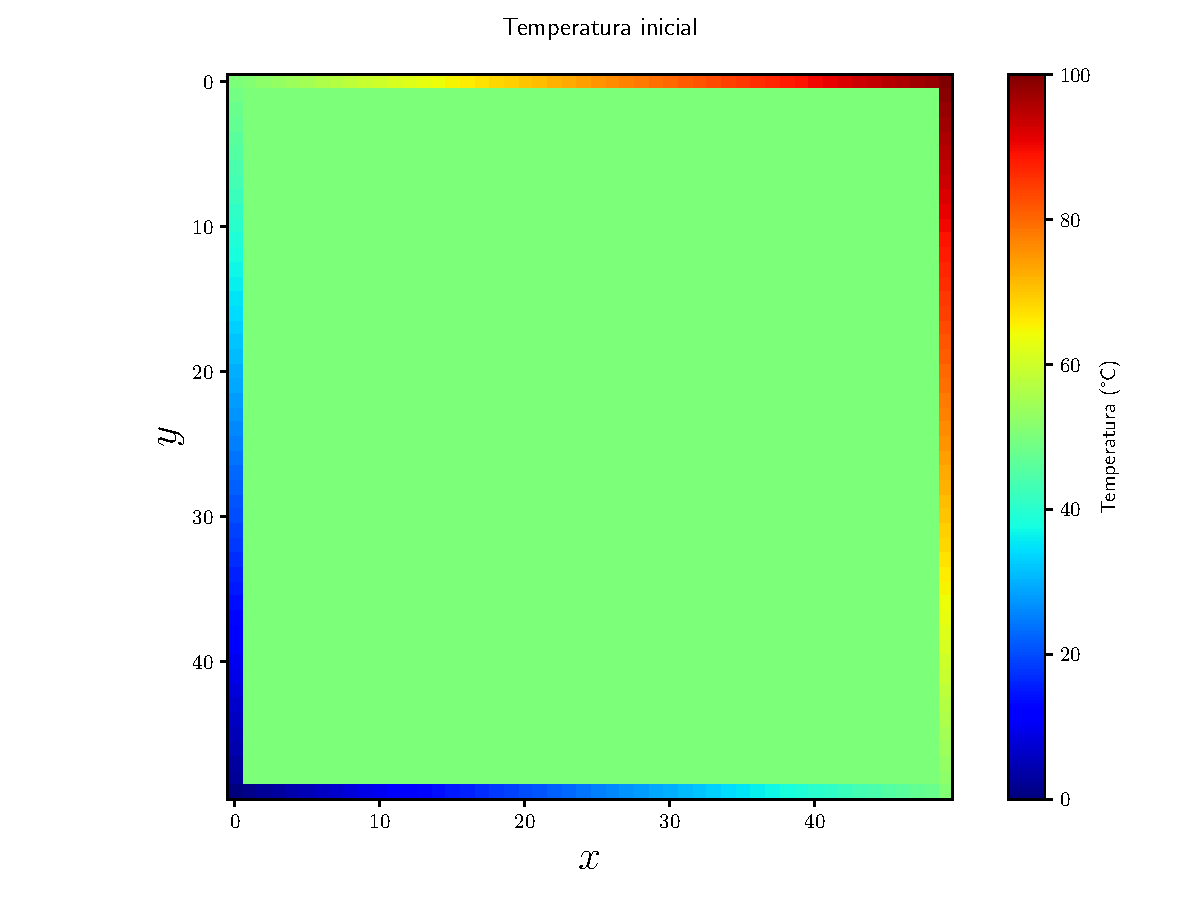
\includegraphics[width=1.0\textwidth]{code/temp-inicial.pdf}
\end{center}

\cw{0.5}
Condiciones de borde:
   \begin{align*}
       u(x, 0) &= 50 + \frac{x (100 - 50)}{L_x}  \\
       u(0, y) &= 50 - y \frac{50}{L_y} \\
    u(x, L_y) &= 50  \frac{x}{L_x} \\
    u(L_x, y) &= 100 - y \frac{50}{L_y} \\
   \end{align*}

Condición inicial:
\[ u(x, y)_{t=0} = 50 \]
\end{columns}
\end{frame}

\begin{frame}
\begin{columns}
\cw{0.45}
\pycode[lastline=18]{code/ec-calor.py}
\cw{0.45}
\pycode[firstline=20, lastline=33]{code/ec-calor.py}
\begin{center}
    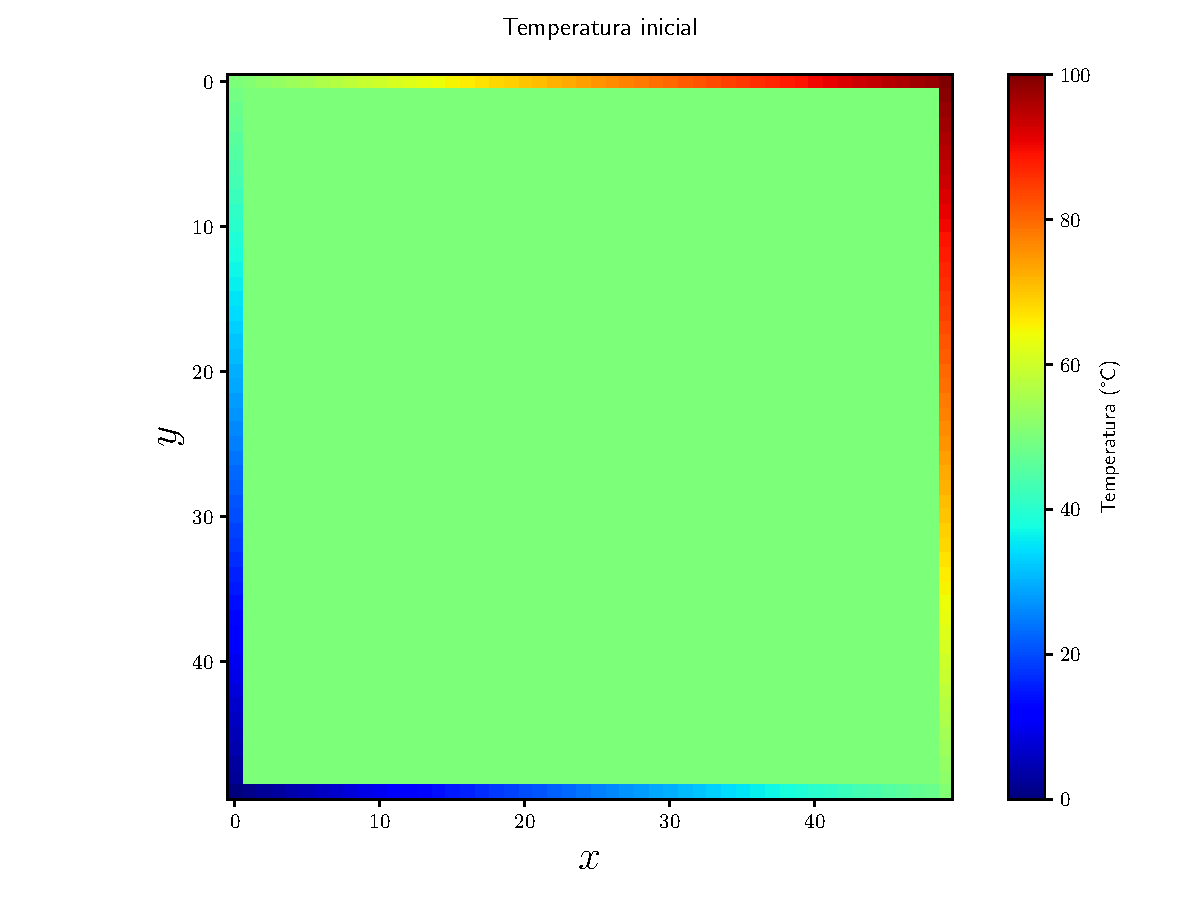
\includegraphics[width=0.7\textwidth]{code/temp-inicial.pdf}
\end{center}
\end{columns}
\end{frame}

\begin{frame}
\begin{columns}
\cw{0.45}
\pycode[firstline=35, lastline=47]{code/ec-calor.py}
\cw{0.45}
%\pycode[firstline=49, lastline=60]{code/ec-calor.py}
\begin{center}
    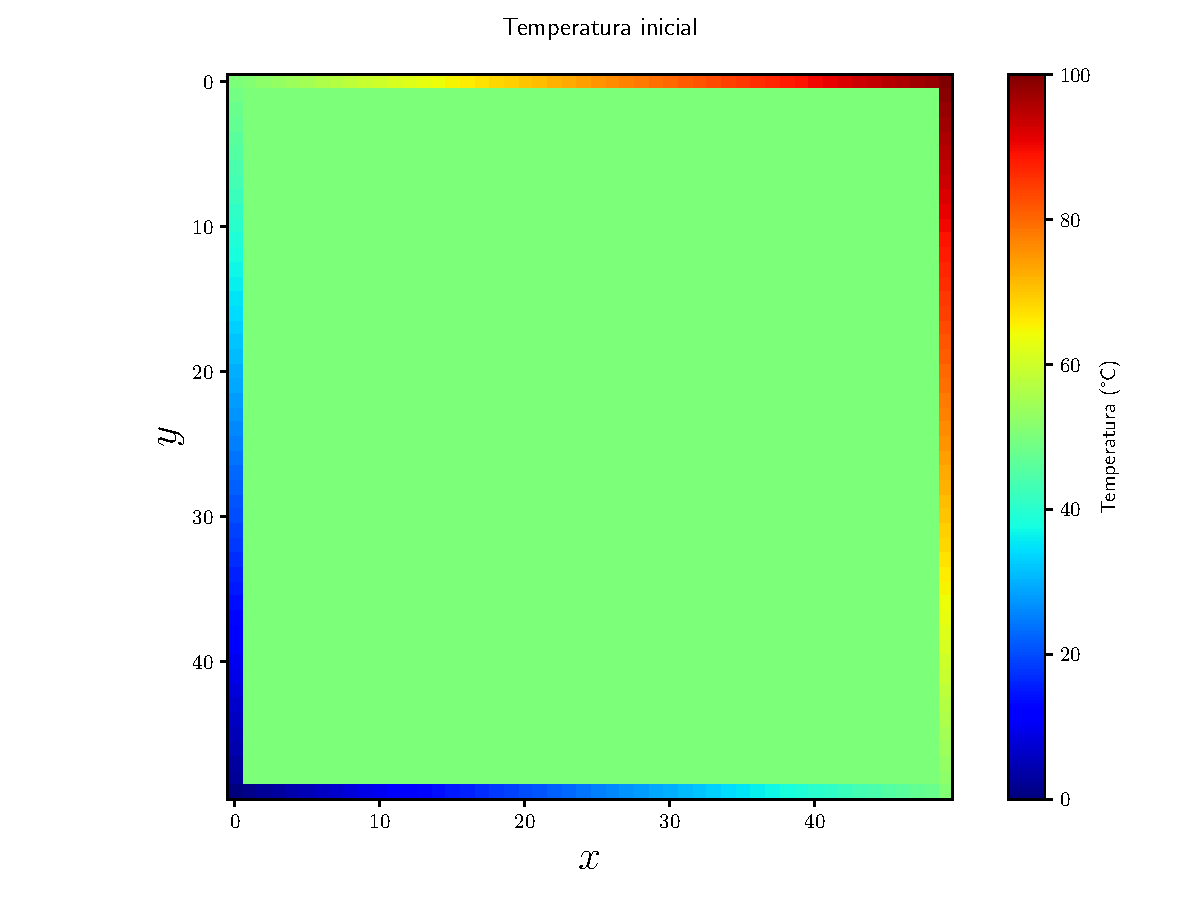
\includegraphics[width=1.0\textwidth]{code/temp-inicial.pdf}
\end{center}
\end{columns}
\end{frame}

\begin{frame}
\begin{columns}
\cw{0.6}
\pycode[firstline=49, lastline=70]{code/ec-calor.py}

\cw{0.38}
\begin{center}
    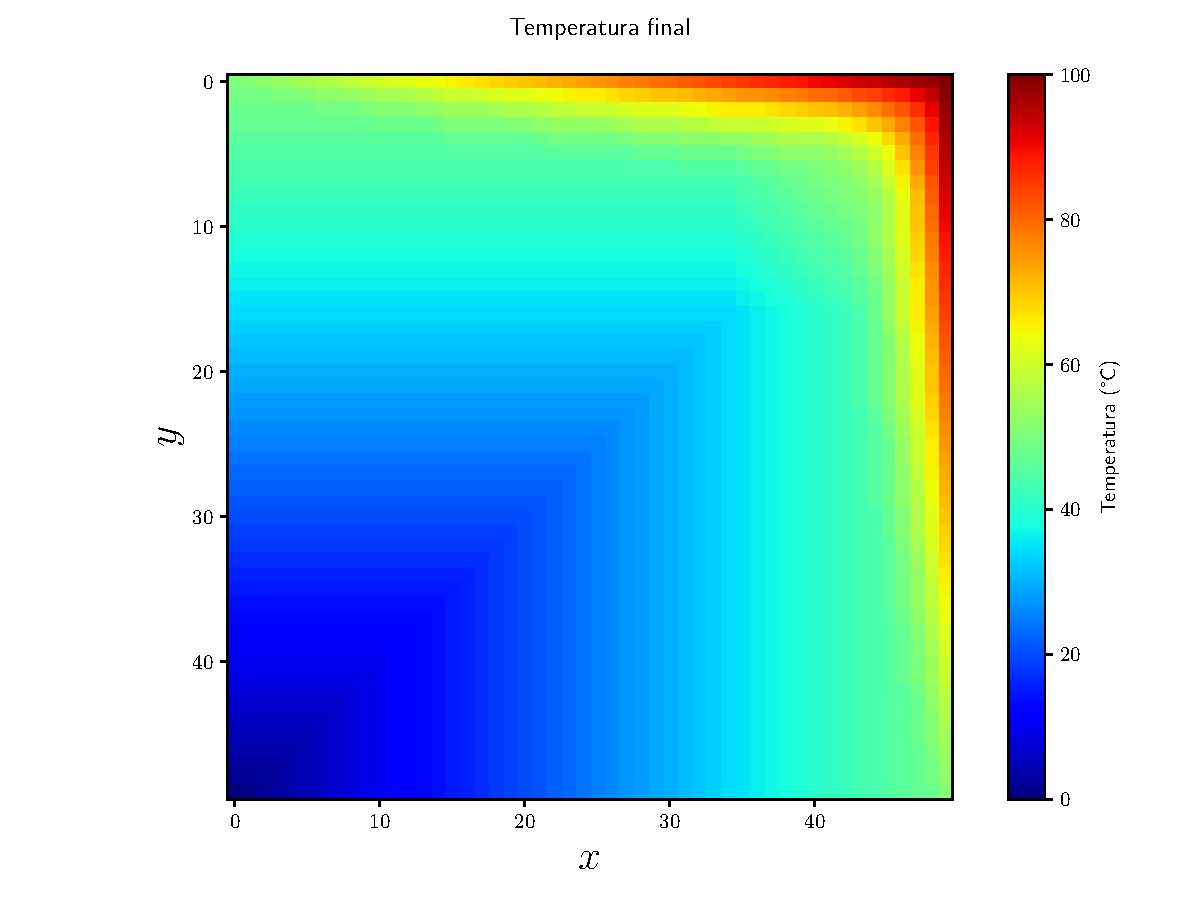
\includegraphics[width=1.0\textwidth]{code/temp-final.pdf}
\end{center}
\end{columns}
\end{frame}

\begin{frame}
\begin{columns}
\cw{0.45}
\pycode[firstline=72, lastline=96]{code/ec-calor.py}
\pause

\cw{0.45}
\begin{center}
 \embedvideo{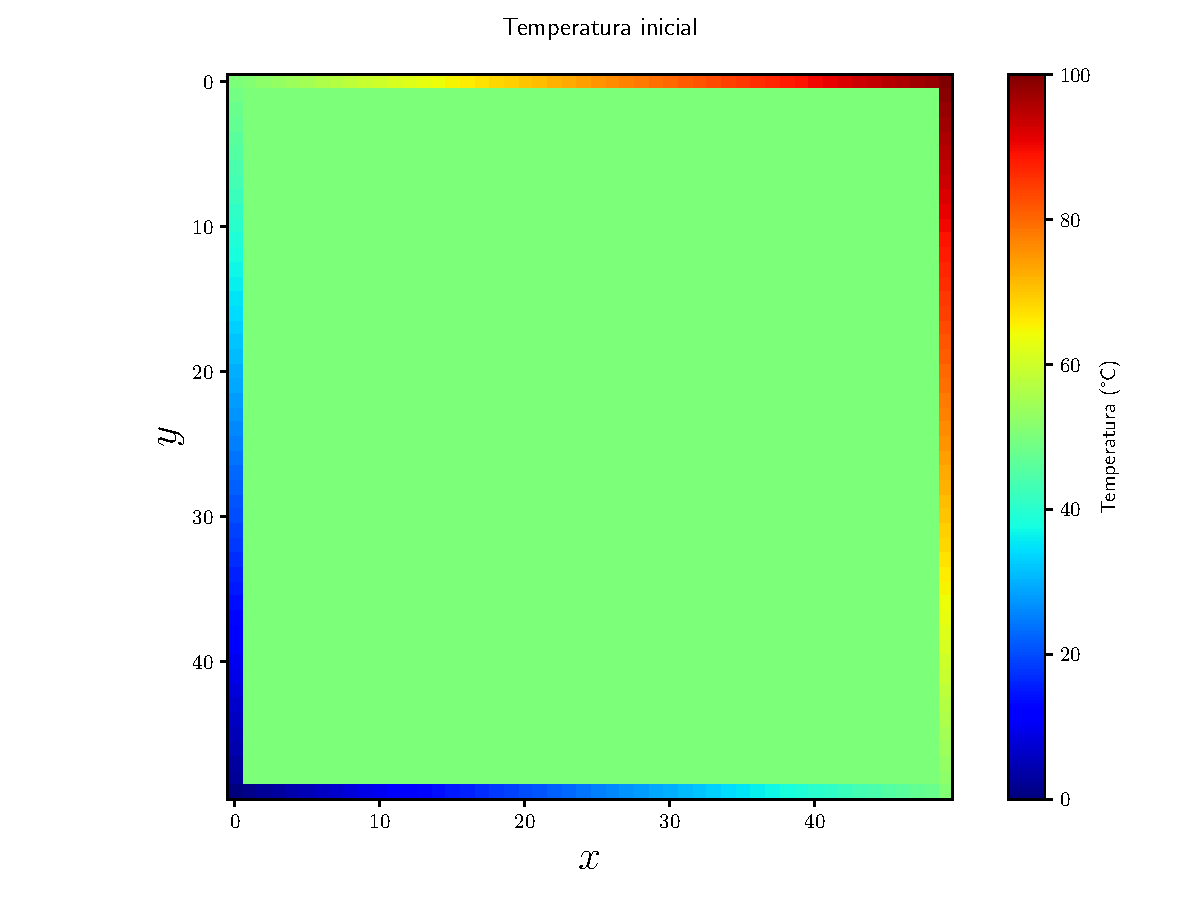
\includegraphics[width=1.0\textwidth]{code/temp-inicial.pdf}}{code/solucion_ecuacion_calor_t.mp4} 
 \end{center}
\end{columns}
\end{frame}

%% Esquema implícito y Crank-Nicolson en Burden 12.2
\begin{frame}
    \begin{columns}[t]
\cx
    \textbf{Análisis de estabilidad:}
\[ \frac{\partial u}{\partial t} (x, t) = \alpha^2 \frac{\partial^2 u}{\partial x^2}(x, t), \; 0 < x < l, \; 0 < t \]
Condiciones de frontera:
\begin{align*}
u(0, t) &= u(l, t) = 0, t > 0; \\
u(x, 0) &= f(x), 0 \leq x \leq l
\end{align*}

Diferencia hacia adelante (o progresiva):
\begin{align*} \frac{\partial u}{\partial t} (x_i, t_j) &= \frac{u(x_i, t_j+k) - u(x_i, t_j)}{k} - \frac{k}{2}\frac{\partial^2 u}{\partial t^2}(x_i, \mu_j) \\
    \frac{\partial^2 u}{\partial x^2} (x_i, t_j) &= \frac{u(x_i+h, t_j) - 2 u (x_i, t_j) + u(x_i-h, t_j)}{h^2}\\ &- \frac{h^2}{12} \frac{\partial^4 u}{\partial x^4}(\xi_i, t_j)
\end{align*}
con $t_j \in(t_j, t_{j+1}), \xi_i \in (x_i, x_{i+1})$
\cx
Resulta:
\[ \frac{u_{i, j+1} - u_{i,j}}{k} - \alpha^2 \frac{u_{i+1, j} - 2 u_{i,j} + u_{i-1,j}}{h^2} = 0 \]
con un error local de truncación:
\[ \epsilon_{i,j} = \frac{k}{2} \frac{\partial^2 u}{\partial t^2}(x_i, \mu_j) - \alpha^2 \frac{h^2}{12} \frac{\partial^4 u}{\partial x^4}(\xi_i, t_j) \]

Solución explícita:
\[ u_{i, j+1}  =\left(1 - \frac{2 \alpha^2 k}{h^2}\right) u_{i,j} + \alpha^2 \frac{k}{h^2} (u_{i+1, j} + u_{i-1, j}) \]
\begin{center}
    \includegraphics[width=0.8\textwidth]{figs/forward}
\end{center}
\end{columns}
\end{frame}

\begin{frame}
\vspace{0.5em}
\begin{columns}[t]
\cx
Matriz $(n-1)\mul(n-1)$:
\[ \bm{A} = \begin{bmatrix}
    (1-2\lambda) & \lambda & 0 & \cdots &  0 \\
    \lambda & (1-2\lambda) & \lambda & \cdots & 0 \\
    0 & \cdots & \cdots & \cdots &  0 \\
    0 & \cdots & \cdots & \cdots &  \lambda \\
    0 & \cdots & 0 & \lambda & (1-2\lambda)
\end{bmatrix} \]

con $\lambda = \alpha^2 k / h^2$

Si $\bm{u^{(0)}} = [f(x_1), f(x_2), \cdots, f(x_{n-1})]^T $, la solución aproximada es:
\[ \bm{u}^{(j)} = \bm{A} \bm{u}^{(j-1)} \]

Supongamos un error $\bm{e}^{(0)} = [e_1^{(0)}, e_2^{(0)}, \cdots, e_{n-1}^{(0)}]^T$:
\[ \bm{u}^{(1)} = \bm{A} (\bm{u}^{(0)} + \bm{e}^{(0)}) = \bm{A} \bm{u}^{(0)} + \bm{A} \bm{e}^{(0)} \]

Para el paso $k$, el error en $\bm{u}^{(k)} = \bm{A}^{k} \bm{e}^{(0)}$. El método es \alert{estable} si $\norm{\bm{A}^{k} \bm{e}^{(0)}} \leq \norm{\bm{e}^{(0)}}$
\[ \norm{\bm{A}^k} \leq 1 \then \rho(\bm{A}^k) = (\rho(\bm{A}))^k \leq 1 \]
\pause

\cx
Autovalores de $\bm{A}$:
\[ \mu_i = 1 - 4 \lambda \pow{\sen\left(\frac{i \pi}{2 n}\right)}{2} \]
Norma $L_{\infty}$:
\[ \rho(\bm{A}) = \max_{1 \leq i \leq n} \abs{1 - 4 \lambda \pow{\sen\left(\frac{i \pi}{2 n}\right)}{2}} \]
que se simplifica a
\[ 0 \leq \lambda \pow{\sen\left(\frac{i \pi}{2n}\right)}{2} \leq \frac{1}{2}, \; i = 1, 2, \ldots, n-1 \]
Esta desigualdad debe valer cuando $h \to 0, n \to \infty$:
\[ \lim_{n\to\infty} \pow{\sen\frac{(n-1)\pi}{2 n}}{2} = 1 \]
Por lo tanto habrá estabilidad si $0 \leq \lambda \leq 1/2$:
\begin{columns}
    \cw{0.4}
\[ \alpha^2 \frac{k}{h^2} \leq \frac{1}{2} \]
\cw{0.6}
$\leftarrow$ \alert{condicionalmente estable}.
\end{columns}
\end{columns}
\end{frame}

\begin{frame}
    \begin{columns}[t]
\cw{0.45}
\textbf{Ejemplo:}
\begin{align*}
\frac{\partial u}{\partial t} (x, t) &= \frac{\partial^2 u}{\partial x^2}(x, t), \; 0 < x < 1, \; 0 < t \\
u(0, t) &= u(1, t) = 0, \quad 0 < t; \\
u(x, 0) &= \sen(\pi x), \quad 0 \leq x \leq 1
\end{align*}
\begin{overprint}
\begin{itemize}
    \item \alert<1>{con $h = 0.1$ y $k = 0.0005$.  (1000 pasos) \\
        \[ \alpha^2 \frac{k}{h} = 0.05 \]} \vspace{-1em}
    \item \alert<2>{con $h = 0.1$ y $k = 0.01$. (50 pasos) \\
        \[ \alpha^2 \frac{k}{h} = 1 \]} \vspace{-2em}
\end{itemize}
\end{overprint}

Solución exacta:
\[u(x, t) = e^{-\pi^2 t} \sen (\pi x) \]

\cw{0.55}
Solución: \texttt{parabolica-progresiva.py}\\[2em]

\begin{overlayarea}{\textwidth}{0.8\textheight}
\begin{center}
\only<1>{\begin{tabular}{ccccc}
\toprule
$i$ & $x_i$ & $u_{i,1000}$ & $u(x_i, 0.5)$ & $\abs{u_{i, 1000} - u(x_i, 0.5)}$ \\
\midrule
0 & 0.0 & 0.00000 & 0.00000 & 0.000e+00 \\
1 & 0.1 & 0.00229 & 0.00222 & 6.411e-05 \\
2 & 0.2 & 0.00435 & 0.00423 & 1.219e-04 \\
3 & 0.3 & 0.00599 & 0.00582 & 1.678e-04 \\
4 & 0.4 & 0.00704 & 0.00684 & 1.973e-04 \\
5 & 0.5 & 0.00740 & 0.00719 & 2.075e-04 \\
6 & 0.6 & 0.00704 & 0.00684 & 1.973e-04 \\
7 & 0.7 & 0.00599 & 0.00582 & 1.678e-04 \\
8 & 0.8 & 0.00435 & 0.00423 & 1.219e-04 \\
9 & 0.9 & 0.00229 & 0.00222 & 6.411e-05 \\
10 & 1.0 & 0.00000 & 0.00000 & 8.808e-19 \\
\bottomrule
\end{tabular} }

\only<2>{\begin{tabular}{ccccc}
\toprule
$i$ & $x_i$ & $u_{i,50}$ & $u(x_i, 0.5)$ & $\abs{u_{i, 50} - u(x_i, 0.5)}$ \\
\midrule
0 & 0.0 & 0.000e+00 & 0.00000 & 0.000e+00 \\
1 & 0.1 & 2.637e+05 & 0.00222 & 2.637e+05 \\
2 & 0.2 & -5.026e+05 & 0.00423 & 5.026e+05 \\
3 & 0.3 & 6.938e+05 & 0.00582 & 6.938e+05 \\
4 & 0.4 & -8.186e+05 & 0.00684 & 8.186e+05 \\
5 & 0.5 & 8.643e+05 & 0.00719 & 8.643e+05 \\
6 & 0.6 & -8.254e+05 & 0.00684 & 8.254e+05 \\
7 & 0.7 & 7.047e+05 & 0.00582 & 7.047e+05 \\
8 & 0.8 & -5.135e+05 & 0.00423 & 5.135e+05 \\
9 & 0.9 & 2.704e+05 & 0.00222 & 2.704e+05 \\
10 & 1.0 & 0.000e+00 & 0.00000 & 8.808e-19 \\
\bottomrule
\end{tabular} }
\end{center}
\end{overlayarea}
\end{columns}
\end{frame}

\begin{frame}
    \begin{columns}[t]
\cx
\textbf{Incondicionalmente estable:} diferencias regresivas (implícito).
\[ \frac{\partial u}{\partial t} (x_i, t_j) = \frac{u(x_i, t_j) - u(x_i, t_{j-1})}{k} - \frac{k}{2}\frac{\partial^2 u}{\partial t^2}(x_i, \mu_j) \]
con $\mu_j \in (t_{j-1}, t_j)$.

Reemplazando en la ecuación en derivadas parciales:
\[ \frac{u_{i,j} - u_{i, j-1}}{k} - \alpha^2 \frac{u_{i+1, j} - 2 u_{i,j} + u_{i-1, j}}{h^2} = 0 \]
para $i = 1, 2, \ldots, n-1$ y $j = 1, 2, \ldots$.
\begin{center}
    \includegraphics[width=0.7\textwidth]{figs/backward}
\end{center} \pause

\cx
Hacemos $\lambda = \alpha^2 k / h^2$:
\[ (1 + 2\lambda) u_{i,j} - \lambda u_{i+1, j} - \lambda u_{i-1, j} = u_{i, j-1} \]
Con las condiciones de frontera:
\begin{align*}
    u_{i, 0} &= f(x_i), \; i = 1, 2, \ldots, n-1 \\
    u_{0, j} &= u_{n, j} = 0, \; j = 1, 2, \ldots 
\end{align*}

Matriz $(n-1)\mul(n-1)$:
\[ \bm{A} = \begin{bmatrix}
    (1+2\lambda) & -\lambda & 0 & \cdots &  0 \\
    -\lambda & (1+2\lambda) & -\lambda & \cdots & 0 \\
    0 & \cdots & \cdots & \cdots &  0 \\
    0 & \cdots & \cdots & \cdots &  -\lambda \\
    0 & \cdots & 0 & -\lambda & (1+2\lambda)
\end{bmatrix} \]
$\bm{u}^{(j)} = [u_{1, j}, u_{2, j}, \cdots, u_{n-1, j}]^T$, $\bm{u}^{(j-1)} = [u_{1, j-1}, u_{2, j-1}, \cdots, u_{n-1, j-1}]^T$
\[ \mapsto \bm{A} \bm{u}^{(j)} = \bm{u}^{(j-1)}, \, j = 1, 2, \ldots \]
\end{columns}
\end{frame}

\begin{frame}
\begin{columns}
\cw{0.45}
\textbf{Ejemplo:} 
\begin{align*}
\frac{\partial u}{\partial t} (x, t) &= \alpha \frac{\partial^2 u}{\partial x^2}(x, t), \; 0 < x < 1, \; 0 < t \\
u(0, t) &= u(1, t) = 0, \quad t > 0; \\
u(x, 0) &= \sen(\pi x), \quad 0 \leq x \leq 1
\end{align*}
con $h = 0.1$ y \alert{$k = 0.01$}.

Solución exacta:
\[u(x, t) = e^{-\pi^2 t} \sen (\pi x) \]
\centering Solución: \texttt{parabolica-regresiva.py}

\cw{0.55}
\begin{center}
\begin{tabular}{ccccc}
\toprule
$i$ & $x_i$ & $u_{i,50}$ & $u(x_i, 0.5)$ & $\abs{u_{i, 50} - u(x_i, 0.5)}$ \\
\midrule
0 & 0.0 & 0.00000 & 0.00000 & 0.000e+00 \\
1 & 0.1 & 0.00780 & 0.00222 & 5.576e-03 \\
2 & 0.2 & 0.01236 & 0.00423 & 8.133e-03 \\
3 & 0.3 & 0.01591 & 0.00582 & 1.010e-02 \\
4 & 0.4 & 0.01817 & 0.00684 & 1.133e-02 \\
5 & 0.5 & 0.01894 & 0.00719 & 1.175e-02 \\
6 & 0.6 & 0.01817 & 0.00684 & 1.133e-02 \\
7 & 0.7 & 0.01591 & 0.00582 & 1.010e-02 \\
8 & 0.8 & 0.01236 & 0.00423 & 8.133e-03 \\
9 & 0.9 & 0.00780 & 0.00222 & 5.576e-03 \\
10 & 1.0 & 0.00000 & 0.00000 & 8.808e-19 \\
\bottomrule
\end{tabular} 
\end{center}
\end{columns} \pause
\vspace{1em}
\begin{columns}
\cx
Autovalores de $\bm{A}$:
\[ \mu_i = 1 + 4 \lambda \left[ \sen \left(\frac{i \pi}{2 n}\right) \right]^2 \]
para $i = 1, 2, \cdots, n-1$. Como $\lambda > 0$, $\mu_i > 0$.

\cx
Entonces $\rho(\bm{A}^{-1}) < 1 \mapsto \bm{A}$ es una matriz convergente:
\begin{columns}
\cw{0.4}
\[ \lim_{j \to \infty} (\bm{A}^{-1})^j \bm{e}^{(0)} = \bm{0} \]
\cw{0.6}
$\leftarrow$ \alert{incondicionalmente estable}.
\end{columns} \pause
\centering Precisión: $\bigO(k + h^2) \leftarrow$ \faThumbsODown
\end{columns}
\end{frame}

\begin{frame}
\begin{columns}
\cx
\textbf{Método de Crank-Nicolson}:

Diferencias progresivas:
\[ \frac{u_{i, j+1} - u_{i,j}}{k} - \alpha^2 \frac{u_{i+1, j} - 2 u_{i,j} + u_{i-1, j}}{h^2} = 0 \]
con error de truncamiento:
\[ \epsilon_p = \frac{k}{2} \frac{\partial^2 u}{\partial t^2}(x_i, \mu_j) + \bigO(h^2) \]

Diferencias regresivas:
\[ \frac{u_{i, j+1} - u_{i,j}}{k} - \alpha^2 \frac{u_{i+1, j+1} - 2 u_{i,j+1} + u_{i-1, j+1}}{h^2} = 0 \]
con error de truncamiento:
\[ \epsilon_r = -\frac{k}{2} \frac{\partial^2 u}{\partial t^2}(x_i, \hat{\mu}_j) + \bigO(h^2) \]
Suponiendo que:
\[ \frac{k}{2} \frac{\partial^2 u}{\partial t^2}(x_i, \mu_j) \approx \frac{k}{2} \frac{\partial^2 u}{\partial t^2}(x_i, \hat{\mu}_j) \]

\cx
el método de la diferencia promediado:
\begin{multline*}
    \frac{u_{i, j+1} - u_{i,j}}{k} - \frac{\alpha^2}{2} \left[ \frac{u_{i+1, j} - 2 u_{i,j} + u_{i-1, j}}{h^2} \right. \\
        + \left. \frac{u_{i+1, j+1} - 2 u_{i,j+1} + u_{i-1, j+1}}{h^2} \right] = 0
\end{multline*}
tiene un error de truncamiento $\bigO(k^2 + h^2) \leftarrow$ \faThumbsOUp

\begin{center}
    \includegraphics[width=0.8\textwidth]{figs/crank-nicolson}
\end{center}
\end{columns}
\end{frame}

\begin{frame}
En forma matricial:
\[ \bm{A} \bm{u}^{(j+1)} = \bm{B} \bm{u}^{(j)}, \txt{para cada} j = 0, 1, \ldots,\txt{donde} \lambda = \alpha^2 \frac{k}{h^2}, \; \bm{u}^{(j)} = [u_{1,j}, u_{2, j}, \cdots, u_{n-1, j}]^T \]
y
\[
\bm{A} = \begin{bmatrix}
    (1+\lambda) & -\lambda/2 & 0 & \cdots &  0 \\
    -\lambda/2 & (1+\lambda) & -\lambda/2 & \cdots & 0 \\
    0 & \cdots & \cdots & \cdots &  0 \\
    0 & \cdots & \cdots & \cdots &  -\lambda/2 \\
    0 & \cdots & 0 & -\lambda/2 & (1+\lambda)
\end{bmatrix} \txt{y}
\bm{B} = \begin{bmatrix}
    (1-\lambda) & \lambda/2 & 0 & \cdots &  0 \\
    \lambda/2 & (1-\lambda) & \lambda/2 & \cdots & 0 \\
    0 & \cdots & \cdots & \cdots &  0 \\
    0 & \cdots & \cdots & \cdots &  \lambda/2 \\
    0 & \cdots & 0 & \lambda/2 & (1-\lambda)
\end{bmatrix}
\]
\end{frame}

\begin{frame}
\begin{columns}
\cw{0.45}
\textbf{Ejemplo:} 
\begin{align*}
\frac{\partial u}{\partial t} (x, t) &= \alpha^2 \frac{\partial^2 u}{\partial x^2}(x, t), \; 0 < x < 1, \; 0 < t \\
u(0, t) &= u(1, t) = 0, \quad t > 0; \\
u(x, 0) &= \sen(\pi x), \quad 0 \leq x \leq 1
\end{align*}
con $h = 0.1$ y \alert{$k = 0.01$}.

Solución exacta:
\[u(x, t) = e^{-\pi^2 t} \sen (\pi x) \]
\centering Solución: \texttt{crank-nicolson.py}

\cw{0.55}
\begin{center}
\begin{tabular}{ccccc}
\toprule
$i$ & $x_i$ & $u_{i,50}$ & $u(x_i, 0.5)$ & $\abs{u_{i, 50} - u(x_i, 0.5)}$ \\
\midrule
0 & 0.0 & 0.00000 & 0.00000 & 0.000e+00 \\
1 & 0.1 & 0.00488 & 0.00222 & 2.660e-03 \\
2 & 0.2 & 0.00812 & 0.00423 & 3.895e-03 \\
3 & 0.3 & 0.01066 & 0.00582 & 4.842e-03 \\
4 & 0.4 & 0.01228 & 0.00684 & 5.436e-03 \\
5 & 0.5 & 0.01283 & 0.00719 & 5.639e-03 \\
6 & 0.6 & 0.01228 & 0.00684 & 5.436e-03 \\
7 & 0.7 & 0.01066 & 0.00582 & 4.842e-03 \\
8 & 0.8 & 0.00812 & 0.00423 & 3.895e-03 \\
9 & 0.9 & 0.00488 & 0.00222 & 2.660e-03 \\
10 & 1.0 & 0.00000 & 0.00000 & 8.808e-19 \\
\bottomrule
\end{tabular} 
\end{center}
\end{columns} 
\end{frame}

\begin{frame}
    \begin{columns}[t]
\cx
\textbf{Ecuación de onda (hiperbólica)}
\[ \frac{\partial^2 u}{\partial t^2} (x, t) - \alpha^2 \frac{\partial^2 u}{\partial x^2}(x, t) = 0, \; 0 < x < l, \; 0 < t \]
Con las ecuaciones de frontera:
\begin{align*}
u(0, t) &= u(l, t) = 0, t > 0; \\
u(x, 0) &= f(x),\; \frac{\partial u}{\partial t}(x, 0) = g(x); \, 0 \leq x \leq l
\end{align*}

Malla:
\[ x_i = i h, \; t_j = j k \]
para $i = 0, 1, \ldots, n$ y $j = 0, 1, \cdots$

En todos los puntos de la malla interior:
\[ \frac{\partial^2 u}{\partial t^2} (x_i, t_j) - \alpha^2 \frac{\partial^2 u}{\partial x^2}(x_i, t_j) = 0 \]

Diferencias centrales para las derivadas segundas:
\cx
\begin{multline*}
    \frac{\partial^2 u}{\partial t^2} (x_i, t_j) = \frac{u(x_i, t_{j+1}) - 2 u(x_i, t_j) + u(x_i, t_{j-1})}{k^2} \\
    - \frac{k^2}{12} \frac{\partial^4 u}{\partial t^4}(x_i, \mu_j)
\end{multline*}
\begin{multline*}
    \frac{\partial^2 u}{\partial x^2} (x_i, t_j) = \frac{u(x_{i+1}, t_j) - 2 u(x_i, t_j) + u(x_{i-1}, t_j)}{h^2} \\
    - \frac{h^2}{12} \frac{\partial^4 u}{\partial x^4}(\xi_i, t_j)
\end{multline*}
donde $\xi_i \in (x_{i-1}, x_{i+1}), \mu_i \in (t_{j-1}, t_{j+1})$. Resulta:
\begin{multline*}
    \frac{u_{i,j+1} - 2 u_{i,j} + u_{i,j-1}}{k^2} \\
    - \alpha^2 \frac{u_{i+1,j} - 2 u_{i,j} + u_{i-1,j}}{h^2} = \epsilon_{i,j}
\end{multline*}
con 
\[ \epsilon_{i,j} = \frac{1}{12} \left[k^2 \frac{\partial^4u}{\partial t^4}(x_i, t_j) - \alpha^2 h^2 \frac{\partial^4 u}{\partial x^4}(x_i, t_j)\right] \]
\end{columns}
\end{frame}

\begin{frame}
\begin{columns}
\cx
Ignorando $\epsilon_{i,j}$ y haciendo $\lambda = \alpha k / h$ (número de Courant):
\[ u_{i, j+1} - 2 u_{i,j} + u_{i, j-1} - \lambda^2 u_{i+1, j} + 2 \lambda^2 u_{i,j} - \lambda^2 u_{i-1, j} = 0 \]

Resolviendo para el paso temporal:
\[ u_{i, j+1} = 2(1 - \lambda^2) u_{i,j} + \lambda^2( u_{i+1, j} + u_{i-1, j}) - u_{i, j-1} \]
para $i = 1, 2, \ldots, n-1$ y $j = 1, 2, \ldots$.

Las condiciones de frontera resultan:
\[ u_{0, j} = u_{n, j} = 0, \; j = 1, 2, \ldots \]
y la condición inicial:
\[ u_{i, 0} = f(x_i), \; i = 1, 2, \ldots, n-1 \]

\cx
\begin{center}
    \includegraphics[width=0.9\textwidth]{figs/hiperbolica.pdf}
\end{center}

Enfoque matricial:
\[ \bm{u}^{(j+1)} = \bm{A} \bm{u}^{(j)} - \bm{u}^{(j-1)} \]
\end{columns}
\end{frame}

\begin{frame}
\[
    \begin{bmatrix} u_{1,j+1} \\ u_{2,j+1} \\ u_{3,j+1} \\ \vdots \\ u_{n-1,j+1} \end{bmatrix}
    =
    \begin{bmatrix}
    2(1-\lambda^2) & \lambda^2 & 0 & \cdots &  0 \\
    \lambda^2 & 2(1-\lambda^2) & \lambda^2 & \cdots & 0 \\
    0 & \cdots & \cdots & \cdots &  0 \\
    0 & \cdots & \cdots & \cdots &  \lambda^2 \\
    0 & \cdots & 0 & \lambda^2 & 2(1+\lambda^2) \end{bmatrix} \;
    \begin{bmatrix} u_{1,j} \\ u_{2,j} \\ u_{3,j} \\ \vdots \\ u_{n-1,j} \end{bmatrix}
    -
    \begin{bmatrix} u_{1,j-1} \\ u_{2,j-1} \\ u_{3,j-1} \\ \vdots \\ u_{n-1,j-1} \end{bmatrix}
\] \pause
\begin{columns}[t]
\cw{0.4}
\alert{Problema:} ¿$u_{i, 1}$? 

Condición de velocidad inicial:
\[ \frac{\partial u}{\partial t}(x, 0) = g(x), \; 0 \leq x \leq l \]
Aproximación por diferencias progresivas:
\[ \frac{\partial u}{\partial t}(x, 0) = \frac{u(x_i, t_1) - u(x_i, 0)}{k} - \frac{k}{2} \frac{\partial^2 u}{\partial t^2}(x_i, \mu_i) \]
Resolviendo:
\[ u(x_i, t_1) = u(x_i, 0) + k g(x_i) +  \frac{k}{2} \frac{\partial^2 u}{\partial t^2}(x_i, \mu_i) \]
Error de truncamiento: $\bigO(k) \leftarrow$ \faThumbsODown
\pause

\cw{0.6}
Mejora: expansión de McLaurin ($\sim$ Taylor):
\[ u(x_i, t_1) = u(x_i, 0) + k \frac{\partial u}{\partial t}(x_i,0) + \frac{k^2}{2} \frac{\partial^2 u}{\partial t^2}(x_i, 0) + \frac{k^3}{6} \frac{\partial^3 u}{\partial t^3}(x_i, \hat{\mu}_i) \]
Si $f''$ existe:
\[ \frac{\partial^2 u}{\partial t^2}(x_i, 0) = \alpha^2 \frac{\partial^2 u}{\partial x^2}(x_i, 0) = \alpha^2 f''(x_i) \]
entonces:
\[ u(x_i, t_1) = u(x_i, 0) + k g(x_i) + \frac{\alpha^2 k^2}{2} f''(x_i) \]
con error $\bigO(k^3) \leftarrow$ \faThumbsOUp. \pause \alert{¿Y si no tenemos $f''(x_i)$?}
\end{columns}
\end{frame}

\begin{frame}
Ecuación en diferencias:
\[ f''(x_i) = \frac{f(x_{i+1}) - 2 f(x_i) + f(x_{i-1})}{h^2} - \frac{h^2}{12} f^{(4)}(\xi_i) \]
Usando $\lambda = \alpha k / h$:
\[ u(x_i, 1) = (1-\lambda^2)f(x_i) + \frac{\lambda^2}{2} f(x_{i+1}) + \frac{\lambda^2}{2} f(x_{i-1}) + k g(x_i) + \bigO(k^3 + h^2 k^2) \]

Entonces, para $i = 1, 2, \ldots, n-1$ usamos:
\[ u_{i, 1} = (1-\lambda^2)f(x_i) + \frac{\lambda^2}{2} f(x_{i+1}) + \frac{\lambda^2}{2} f(x_{i-1}) + k g(x_i) \]
y la ecuación matricial para $j = 2, 3, \ldots$

\end{frame}

\begin{frame}
\begin{columns}
    \cw{0.4}
\texttt{hiperbolica.py}
\pycode[firstline=6, lastline=27]{code/hiperbolica.py}
\pause

\cw{0.5}
\begin{center}
    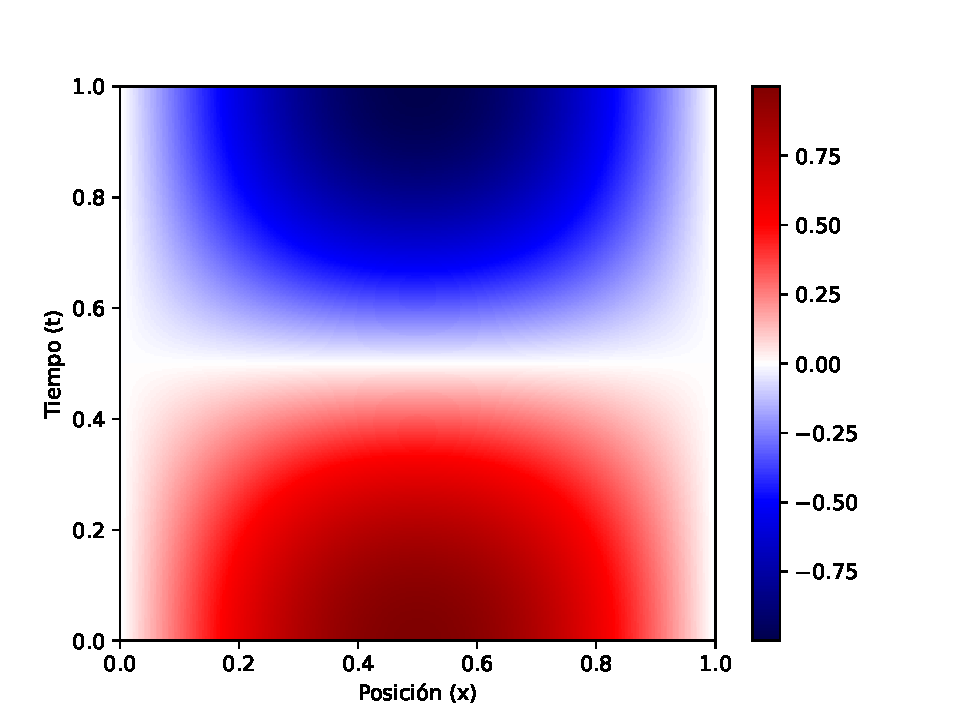
\includegraphics[width=0.7\textwidth]{code/onda-1.pdf}
    \includegraphics[width=0.7\textwidth]{code/onda-2.pdf}
\end{center}
\end{columns}
\end{frame}

\section*{Bibliografía}
\begin{frame}[allowframebreaks]{Lecturas recomendadas}
\begin{itemize}
    \item \fullcite{burden2017}. Capítulo 12.
    \item \fullcite{nakamura1992}. Capítulos 11, 12 y 13.
\item \fullcite{kreyszig2011}. Capítulo 21.
    \item \fullcite{langtangenLinge2016}. Capítulo 3.
\end{itemize}
\end{frame}

\end{document}

